% !TEX root = ../main.tex

\secc[Context]{Context and scope of the project}
\ssecc{Context}

Nowadays one of the most extensive uses of computing is artificial intelligence. A few 
examples are Amazon purchase recommendations, based on previous purchases, or help users
to interact with their phone by only using voice commands like Google Assistant 
~\cite{neural:amazon, neural:google-assistant}.

Inside AI one of the domains that has greatly increased during the last years is 
\gls{ML}. The main advantage of those unsupervised techniques is that it can solely 
learn from examples without explicit teaching, and thus reducing the human interaction 
during the learning process. One of the most used tools is \emph{deep neural networks} 
and these have demonstrated impressive performance with computer vision and Natural 
Language Processing tasks like the classification of digits from the MNIST data set
~\cite{neural:mnist, neural:empirical-evaluation-deep-architectures}.

Regarding the Information Systems in Medicine, recent deep learning al\-go\-ri\-thms, specially 
\gls{CNN} have started to push the boundaries of \gls{precision-medicine}, which is an
emerging approach for disease treatment and prevention that takes into account individual 
variability in genes, environment and lifestyle for each person
~\cite{neural:precision-medicine}. Traditionally, medical 
predictions have been based on a few clinical parameters with poor accuracy.
However, other data types are available to improve such predictions. In this context, 
medical images generated from \gls{MRI}, \gls{PET} or \gls{CT} scans are vastly 
underused due to the inability of radiologists to quantitatively analyze these 
complex data.

Different methods have appeared to analyze these images for tasks such as image 
classification, object detection, segmentation and registration among other tasks. This
approach started in the late 1990s and has slowly shifted from systems that are 
completely designed by humans to systems that are trained by computers using example data
~\cite{medical:survey-deep-learning}.

High-dose radiotherapy with or without chemotherapy is the standard of care for many
locally advanced cancers, like \emph{oropharynx cancer}. While effective in some patients,
these treatments are associated with significant risks of early and late toxicities
that impair patients' treatment adherence and long-term quality of life. Furthermore, 
most cancers are currently treated with a one-size-fits-all approach that invariably leads
to over-treatment of some patient and under-treatment of others. 
The clinical implication of this is that some patients are cured by the standard 
one-size-fits-all treatments currently employed while others are not 
~\cite{medical:personalized}. Refined prognostic 
models are needed to assist clinicians in delivering the appropriate level of care.

Professor Benjamin Haibe-Kains has participated in one of the seminal studies in 
\emph{Radiomics} (Nat Comm). Radiomics is a new emerging field of research that can 
non-invasively quantify tumour phenotypes, based on mining and extracting a large 
number of quantitative imaging features
~\cite{medical:radiomics:data, medical:radiomics:extract-information}.
It is aimed at using computational techniques to extract
the most informative features from radiological images routinely used in clinical settings.
Recent studies have demonstrated the effectiveness of radiomic features as biomarkers 
associated with survival of patients with lung and head and neck cancers. Conventional
radiomic pipelines comprise four main components:
\begin{itemize}
  \item Image acquisition
  \item Extracting hand-engineered features
  \item Assessing their robustness
  \item Building predictive models based on the most relevant features
\end{itemize}

Different machine learning approaches, such as \glspl{NN}, have been applied for the last 
step of the pipeline. However, recent advances have allowed for more complex (deeper) 
\glspl{NN}, and have led to unique feature learning properties with unprecedented performance
for image classification. Contrary to the conventional radiomic models, deep learning methods
are end-to-end and eliminate the need for hand-engineered features, which may not necessarily 
be the most relevant set of features for prognostication of cancer patients.
~\cite{medical:radiomics-ml-classifiers}.

As these data treats with patients' survival, survival analysis methods are required to 
be able to analyze and deal with issues related with survival data, such as patient 
censoring and hazard prediction.


\sssecc{Survival Analysis}
\label{sec:survival}

Survival Analysis is a branch of statistics that analyzes the duration time of the observed
events. Typically it refers to the time to the failure of a physical component or to death of a
patient. It usually defines the following terms~\cite{neural:survival-analysis-1}:

\begin{description}
  \item[\Gls{event} \glssymbol{event}] \glsdesc*{event}
  \item[\Gls{time} \glssymbol{time}] \glsdesc*{time}
  \item[\Gls{baseline} \glssymbol{baseline}] \glsdesc*{baseline}
  \item[\Gls{censoring}] \glsdesc*{censoring}
\end{description}

The survival and hazard functions are the two fundamental functions in survival analysis
~\cite{medical:cox}. The survival function \( S(t) = \Pr(T \ge t) \), is the probability that 
an individual has \emph{survived} beyond time \( t \). The hazard function \( \lambda(t) \) 
is a measure of risk at time \( t \) and it's defined as:
\[
  \lambda(t) = \lim_{\Delta t \rightarrow 0}
  \frac{\Pr(t \le T < t + \Delta t | T \ge t)}{\Delta t}
\]

Usually, when trying to fit a survival model a \gls{CPH} model is used. This type of model
intends to use the \gls{baseline} \( \bm{x} = (x_1, x_2, ..., x_p) \)
to fit the hazard function \( \lambda(t) \)
in the following way:
\[
  \lambda(t | \bm{x}) = \exp(\bm{x}\bm{\beta}) \cdot \lambda_0 (t)
\]
Where \( \bm{\beta} \) is a \( p \times 1 \) vector of unknown parameters, that need to be fit, 
and \( \lambda_0(t) \) is an unknown function giving the standard set of conditions 
\( \bm{x} = \bm{0} \). As it can be seen this model requires for a log-linear relation between
the \gls{baseline} \glssymbol{baseline} and the hazard function \( \lambda(t | \bm{x}) \).

However, casting the survival analysis as a ranking problem is a way of dealing with the biased
distributions of survival times and the censoring data. Two subjects' survival times can be 
ordered only if:
\begin{itemize}
  \item Both of them are uncensored (\( \bm{E}_i = \bm{E}_j = 1\))
  \item The uncensored time of one is smaller than the censored survival time of the other
  (\( \bm{T}_i < \bm{T}_j | \bm{E}_i = 1; \bm{E}_j = 0 \))
\end{itemize}

This can be visualized by means of an order graph \( G = (V, E) \), see \autoref{fig:graph-ci}.
The set of vertices \( V \) represents all the individuals, where each filled circle 
(\( \bullet \)) indicates an \emph{uncensored} survival time, while an empty circle 
(\( \circ \)) denotes a \emph{censored} observation.
Existence of an edge \( E_{ij} \) implies that \( \bm{T}_i < \bm{T}_j \). An edge cannot originate 
from a censored point.

\begin{figure}
  \centering
  \begin{subfigure}[b]{.4\textwidth}
    \centering
    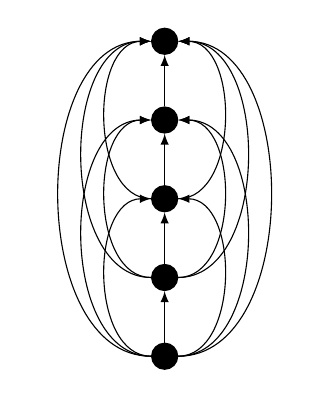
\begin{tikzpicture}
  \tikzstyle{bDot}=[circle, fill=black, draw]
  \foreach \y in {1,...,5} {
    \node[bDot] (D-\y) at (0, \y) {};
  }

  \foreach \y in {1,...,4} {
    \pgfmathsetmacro{\z}{int(\y + 1)}
    \draw[-latex] (D-\y) -- ({D-\z}.south);
  }

  \foreach \y in {1,...,3} {
    \pgfmathsetmacro{\z}{int(\y + 2)}
    \foreach \j in {\z,...,5} {
      \ifthenelse{\y=2 \OR \y=3}{
        \draw[-latex] (D-\y) to[bend left=90] (D-\j);
      }{
        \draw[-latex] (D-\y) to[bend right=90] (D-\j);
      }
    }
  }
\end{tikzpicture}

    \caption{Without censored data}
  \end{subfigure}
  ~
  \begin{subfigure}[b]{.4\textwidth}
    \centering
    \begin{tikzpicture}
  \foreach \y in {1,...,5} {
    \ifthenelse{\y=2 \OR \y=4}{
      \node [circle, fill=white, draw=black] (D-\y) at (0, \y) {};
    }{
      \node [circle, fill=black, draw=black] (D-\y) at (0, \y) {};
    }

    \foreach \y in {3,4,5} {
      \draw [-latex] (D-1) to[bend right=90] (D-\y);
    }

    \foreach \y/\z in {1/2, 3/4} {
      \draw [-latex] (D-\y) -- (D-\z);
    }
    \draw [-latex] (D-3) to[bend left=90] (D-5);
  }
\end{tikzpicture}

    \caption{With censored data}
    \label{fig:graph-ci:censored}
  \end{subfigure}

  \caption[Order graph with ranking constraints]{
    Order graphs representing the ranking constraints \label{fig:graph-ci}
    
    Censored data is represented by \( \circ \) and uncensored data is represented by \( \bullet \).
    Every edge \( A \rightarrow B \) means \( T_A > T_B \). Note that in 
    \autoref{fig:graph-ci:censored} some vertex are not connected since an edge 
    \( \circ \rightarrow \bullet \) cannot be formed.
  }
\end{figure}

% C-index explanation
The standard performance measure, to compare if a survival 
model is performing better than another, is the \gls{CI}. To obtain this 
indicator, pairs are generated to compare the survival time. A prediction is counted as good only
if both \( T_i > T_j \) and \( \hat{T}_i > \hat{T}_j \), otherwise
it's counted as a bad prediction, note that \( T_i = \hat{T}_i \) it's not a required condition. 
Then, the number of good predictions is divided by the total predictions. 
~\cite{medical:ranking-ci}

\[
  CI = \frac{\text{Good predictions}}{\text{Total predictions}} \in [0, 1]
\]

Also, another comparison 
element is the \gls{ROC} curve which represents the \emph{False Positive Rate} against the 
\emph{True Positive Rate}, see \autoref{fig:ROC-curve}. Usually the \gls{CI} is seen as 
the area under the \gls{ROC} curve.
~\cite{neural:roc-precision-recall}

\begin{figure}
  \centering
  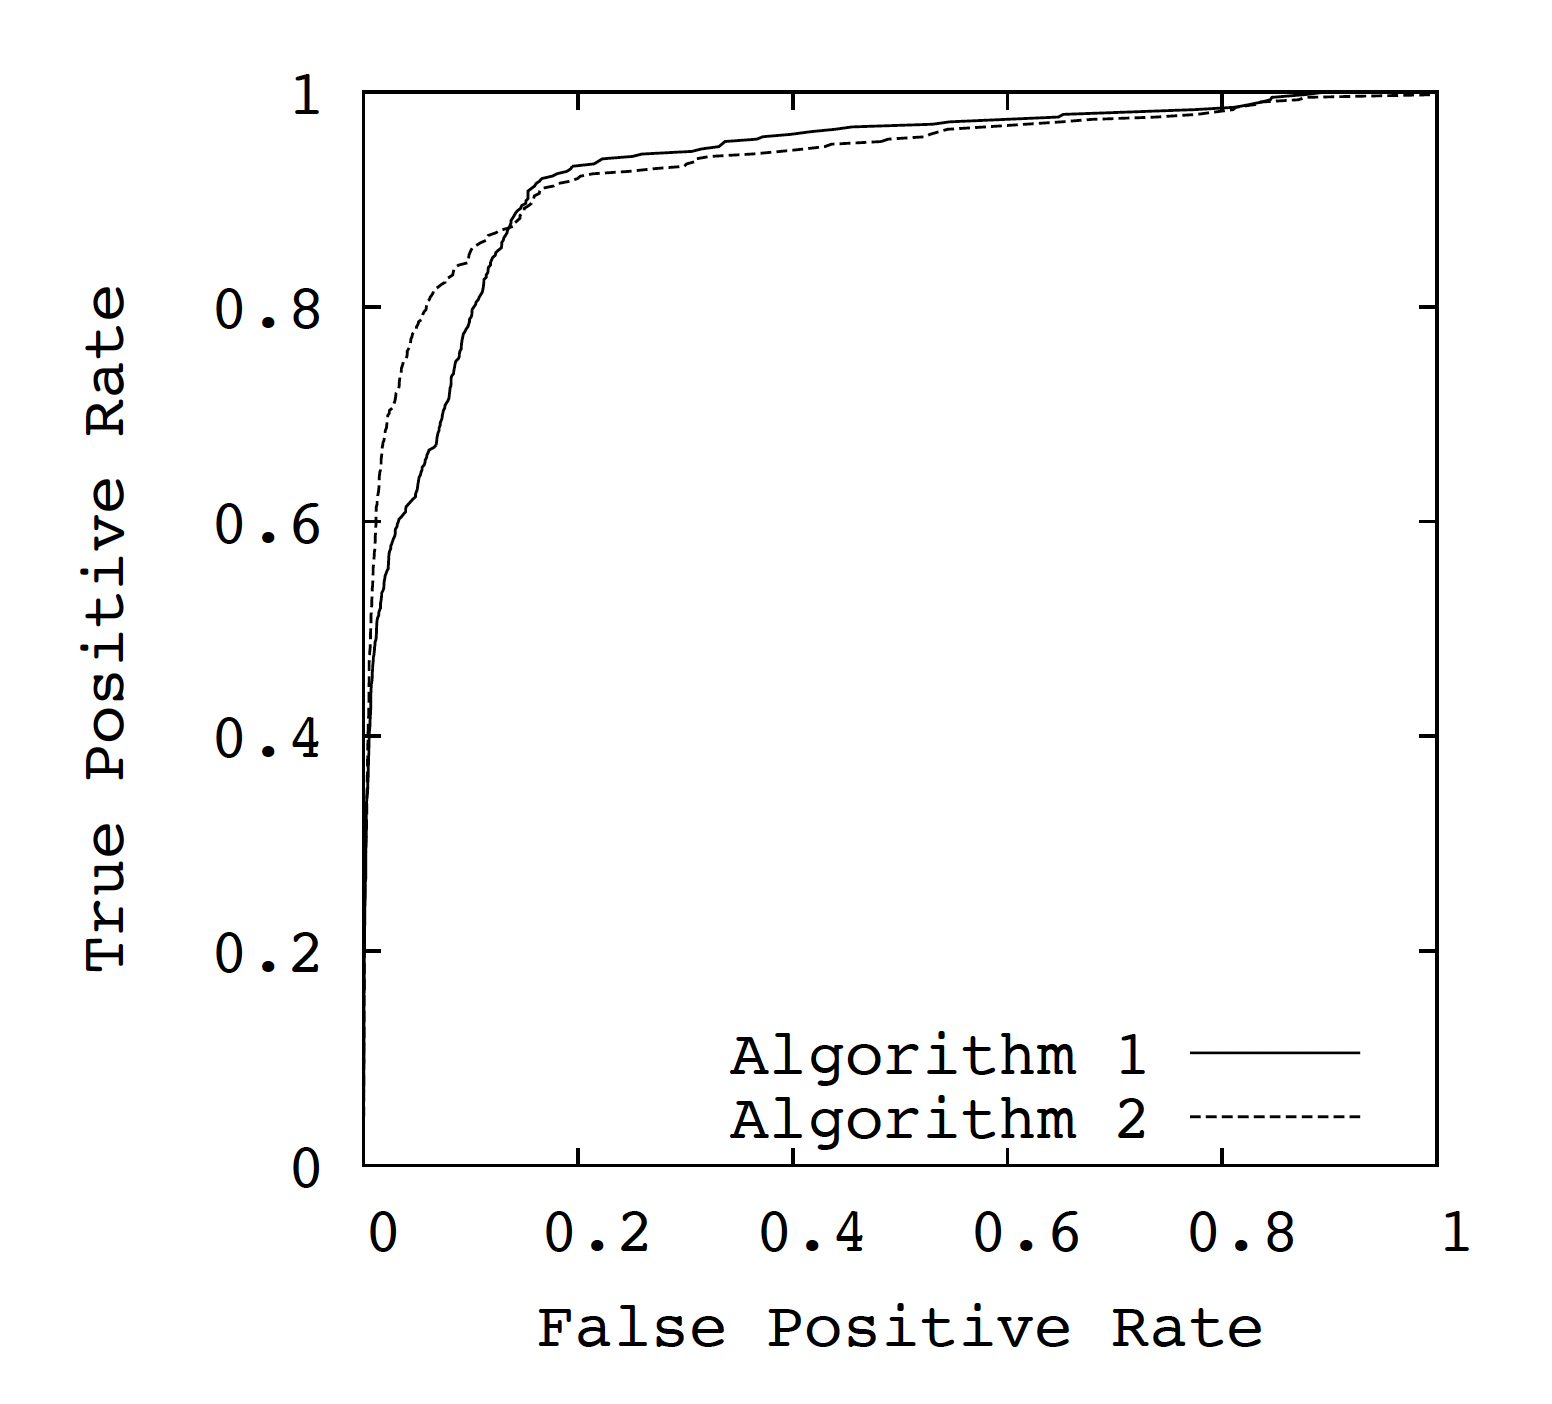
\includegraphics[width=.5\linewidth]{images/roc_curve}
  \caption{\acrshort{ROC} Curve example\label{fig:ROC-curve}}
\end{figure}

\sssecc{Dataset}

The dataset used by this project to develop a model is provided through a 
collaboration with Dr.~Fei-Fei Liu, head of the Radiation Medicine Program at Princess
Margaret Cancer Centre.

We have access to a unique set of 671 cancer patients diagnosed of \gls{OPSCC}. Accounting
for approximately half a million cases annually worldwide, \gls{HNSCC} 
is a considerable cause of mortality and morbidity, with the majority of patients having
locally advanced, unresectable disease. \gls{OPSCC} has been one of the fastest growing 
disease sites for \gls{HNSCC}.
~\cite{medical:ct-based-radiomic-signature}

Multiple information is provided for each patient. There's a \gls{CT} scan, where the tumour 
can be seen, and clinical information about the patient. The scan is 512 pixels wide by 512 
pixels tall and is composed of 100-200 slices in gray scale that together form a 3D image. 
To be able to slice the tumour from the rest of the image, a mask of the same size as the scan 
is provided. The masks contains information about the tumour location, it has \texttt{1}s 
in the pixels containing the tumour and \texttt{0}s
otherwise, as it can be seen in \autoref{fig:dataset-example}.

In the following document we will be calling this the \gls{PMHNK} dataset.

Regarding the clinical information the following fields are provided:
\begin{itemize}
  \item Subject characteristics (age, gender, clinical status, smoking, drinking history)
  \item Tumor characteristics (cancer location, staging, p16 status)
  \item Treatment data (modality, radiation start/end dates, radiation dose/fractionation, 
  treatment completion status)
  \item Outcome data (status, cause of death, local failure, regional failure, distant failure)
\end{itemize}

\begin{figure}
  \centering
  \begin{subfigure}[t]{.32\textwidth}
    \centering
    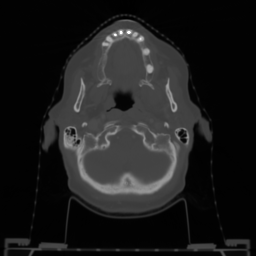
\includegraphics[width=\textwidth]{images/IMG0138_example.png}
    \caption{Original image}
  \end{subfigure}
  \hfill
  \begin{subfigure}[t]{.32\textwidth}
    \centering
    
\includegraphics[width=\textwidth]{images/IMG0138_MASS_example.png}
    \caption{Image mask}
  \end{subfigure}
  \hfill
  \begin{subfigure}[t]{.32\textwidth}
    \centering
    
\includegraphics[width=\textwidth]{images/IMG0138_merge_example.png}
    \caption{Mask applied to original}
  \end{subfigure}

  \caption[Images from the dataset]{
    Example of images from the dataset \label{fig:dataset-example}
    
    Single \gls{CT}'s scan slice, a whole scan is composed of multiple slices. By applying 
    the mask to the original image, the part that only contains the tumour can be extracted.
  }
\end{figure}


\sssecc{Neural Networks}

Neural Networks are a class of \gls{ML} algorithms. The idea is to extract multiple 
linear combinations of the inputs as derived features and model the objective as a nonlinear
function of these features. As it has been previously explained this is a powerful learning
method which has had really good results in many fields.
~\cite{neural:elements-statistical-learning}

A neural network is a two-stage regression or classification algorithm, typically represented
by a graph (or network) diagram as seen in \autoref{fig:neural_network}. It is composed by 
\( L \) layers and each layer has multiple units. The number of units in layer \( l \) 
is defined by  \( n^{[l]} \).

Each hidden unit has an activation (output) computed in two steps, the linear and the 
non-linear step, these are represented by \( \bm{z} \) and \( \bm{a} \) respectively.
These are called hidden units because the values of \( \bm{z} \) and \( \bm{a} \) are 
not directly observed. In general, more than one hidden unit is used to fit more complex 
features.

The linear step is performed by adding each output from the
previous layer (\( l - 1 \)), multiplying it by a weight and adding a bias.
Here, \(w_{ij}^{[l]}\) denotes a weight between unit \( j \) of layer \( l - 1 \) 
and unit \( i \) of layer \( l \). 

The non-linear step is defined by applying a non-linear function, called activation, 
(\( g^{[l]} \)) to the linear part. 
Multiple activation functions can be seen in \autoref{fig:activation_functions}. Depending
on the application, a different activation function may be used, for example in 
\glspl{CNN} usually the ReLU function is used due to the low computational complexity. 
These are defined as:
~\cite{neural:bishop}
\begin{itemize}[itemsep=1ex]
  \item Rectified Linear Unit function 
  \( g(x) = \max(0, x) \)
  \item Hyperbolic tangent function 
  \( \displaystyle g(x) = \tanh(x) = \frac{e^x - e^{-x}}{e^x + e^{-x}}\)
  \item Logistic function 
  \( \displaystyle g(x) = \frac{1}{1 + e^{-x}} \)
\end{itemize}

So, the whole activation for unit \( i \) of layer \( l \) is as follows:
\begin{align*}
  z_i^{[l]} &= \sum_{j = 1}^{n^{[l]}} w_{ij}^{[l]} + w_{i0}^{[l]} \cdot a_j^{[l - 1]} \\
  a_i^{[l]} &= g^{[l]}(z_i^{[l]})
\end{align*}

By using a matrix notation, it can be applied to the whole layer's units:
\begin{align*}
  \bm{z}^{[l]} &= \bm{W}^{[l]} \cdot \bm{a}^{[l - 1]} + \bm{b}^{[l]} \\
  \bm{a}^{[l]} &= g^{[l]}(\bm{z}^{[l]})
\end{align*}


\begin{figure}
  \centering
  \tikzset{
  pics/layer/.style n args = {3}{
    code = {
      \ifthenelse{\equal{#3}{H}}{
        \def\cellcolor{red!20}
      }{
        \ifthenelse{\equal{#3}{I}}{
          \def\cellcolor{green!20}
        }{
          \def\cellcolor{Cyan!20}
        }
      }

      \foreach \y in {1,...,#1} {
        \node[draw, circle, fill=\cellcolor] 
          (L-#2-\y) at (0,{1.5*(#1/2 - \y)}) {${#3}_{\y}^{[#2]}$};
      }
    }
  }
}

\begin{tikzpicture}

\def\layers{2/I, 4/H, 4/H, 3/O}

\foreach \x/\name [count=\xi] in \layers  {
  \draw (3*\xi, 0) pic {layer={\x}{\xi}{\name}};
}

\foreach \x/\ignore [count=\xi, remember=\xi as \lastxi, remember=\x as \lastx] in \layers {
  \ifthenelse{\xi > 1}{
    \foreach \ylast in {1,...,\lastx} \foreach \y in {1,...,\x}{
      \draw [-latex] (L-\lastxi-\ylast) -- (L-\xi-\y);
    }
  }{};
}

\draw (L-1-1) -- (L-2-1) node[midway, sloped, above] {\( w_{ij} \)};

\end{tikzpicture}


  \caption[Neural network graph]{
    Neural Network graph drawing. 
    \label{fig:neural_network}
    
    Each circle represents a unit, green means input, red hidden and blue a output unit.
    In this case the network has 2 units for the input layer, 2 hidden layers with 4 units
    each and 3 units in the output layer.

    Each arrow represents a weight $w_{ij}^{[l]}$ between two units.
  }
\end{figure}
\begin{figure}
  \centering
  
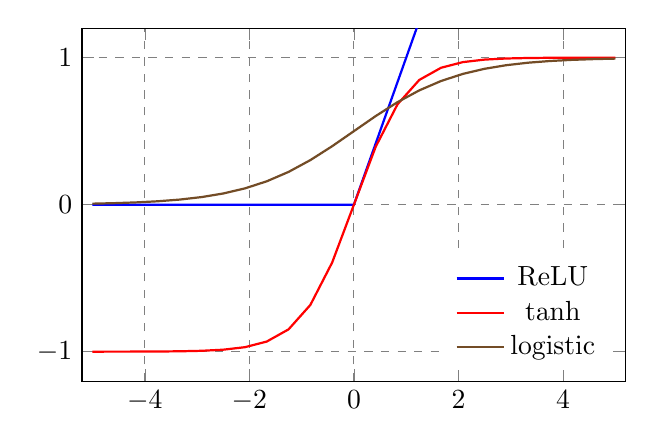
\begin{tikzpicture}
\begin{axis}[
    xmin = -5.2, xmax = 5.2,
    ymin = -1.2, ymax = 1.2,
    legend style = {draw = none},
    legend pos = south east,
    grid=major,
    grid style = {dashed, gray},
    width = 0.7\textwidth,
    height = 0.5\textwidth,
    every axis plot/.append style={thick},
    no markers,
    cycle list name = color
  ]
  \addplot{max(0, x)};
  \addplot{tanh(x)};
  \addplot{1/(1 + exp(-x))};
  \legend{ReLU, tanh, logistic}
\end{axis}
\end{tikzpicture}

  \caption[Activation functions]{
    Activation functions.
    \label{fig:activation_functions}
  }
\end{figure}

The output units allow for a final transformation of the previous layer's vector of outputs.
For regression, typically the identity function \( g^{[L]}(\bm{a^{[L - 1]}}) = \bm{a^{[L - 1]}} \)
is chosen. However, if \( K \)-class classification is going to be used usually the
\emph{softmax} function is used instead. This function provides a probability for each
one of the \( K \) classes:
\[
  g_k^{[L]}(\bm{a}^{[L - 1]}) = \frac{e^{a_k^{[L - 1]}}}{\sum_{i = 1}^K e^{a_i^{[L - 1]}}}
\]

As it has been said, a \gls{NN} has unknown parameters \( \bm{W}^{[l]} \), called weights, and the objective is
to find the values that make the model fit the training data well. The cost function 
is the objective function to be minimized, for regression it's usually defined as 
the mean squared error:

\begin{align*}
  \hat{\bm{y}} &:= g^{[L]}(\bm{a^{[L - 1]}}) \\
  C(\bm{y}, \hat{\bm{y}}) &:= \frac{1}{N} \sum_{i = 1}^N (y_i - \hat{y}_i)^2
\end{align*}

To minimize the objective function, the gradient descent algorithm is used. It is an iterative
algorithm that updates the weights by partial derivative of the cost function with respect to 
the weight. The amount to be updated is defined by the learning rate \( \alpha \):
\begin{align*}
  \underbrace{w_{ij}^{[l]}}_{\text{new}} = \underbrace{w_{ij}^{[l]}}_{\text{old}} - \alpha 
  \frac{\partial C(\bm{y}, \hat{\bm{y}})}{\partial w_{ij}^{[l]}}
\end{align*}

To update all the network's parameters the back-propagation algorithm is used. It's based
in the chain rule derivative and it updates the parameters from the last layer to the first
one.
~\cite{neural:efficient-backprop}


\sssecc{Convolutional Neural Networks}

\glspl{CNN} are a subset of \glspl{NN}. These networks are used for tasks such as 
computer vision due to the high accuracy that can be achieved in image recognition problems.
They can be accelerated through hardware such as \glspl{GPU}. Even though they can be used 
without \glspl{GPU} the operations can be really optimized by these type of processors. 

The convolution operator is denoted by \( * \). In \gls{ML}, the input is usually 
a multi-dimensional array and the convolution kernel is usually another multi-dimensional
array of parameters that are learned by the learning algorithm. When working with 
convolutions, the kernel matrix is flipped before performing the operations. However,
many \gls{NN} libraries perform the cross-correlation operation, which is the same
but without flipping the kernel. A graphical example of the convolutional operation 
can be seen in \autoref{fig:conv-operation}.
~\cite{neural:deeplearning-book}

Usually, a convolutional layer is defined by four parameters:
\begin{description}[topsep=0em]
  \item[Padding] \( p \) amount of extra space added around the matrix being convoluted, 
  usually in form of 0s. This defines the following terms:
  \begin{description}
    \item[Same] Add padding so the output size ends up being the same as the input size
    \item[Valid] Do not add padding at all
  \end{description}
  \item[Stride] \( s \) displacement of the filter
  \item[Filter size] \( f \) size of the filter matrix, usually it has the same width as height but
  it's not mandatory.
  \item[Number of filters] amount of different kernels that will be used to filter the input
  image to generate multiple images as output. It can be seen as filtering first the 
  vertical lines, then the horizontal ones and so on.
\end{description}

Having all the parameters, if one of the dimension's input size is \( n_{\text{prev}} \)
the output size will be defined by:
\begin{align*}
  n_{\text{next}} = \left\lfloor\frac{n_{\text{prev}} + p - f}{s}\right\rfloor + 1
\end{align*}

\begin{figure}
  \centering
  
\usetikzlibrary{matrix, positioning}
\begin{tikzpicture}
  \matrix (mtr) [matrix of nodes,row sep=-\pgflinewidth, nodes={draw}]
	{
		0 & 1 & 1 & |[fill=red!30]| 1 & |[fill=red!30]| 0 & |[fill=red!30]| 0 & 0\\
		0 & 0 & 1 & |[fill=red!30]| 1 & |[fill=red!30]| 1 & |[fill=red!30]| 0 & 0\\
		0 & 0 & 0 & |[fill=red!30]| 1 & |[fill=red!30]| 1 & |[fill=red!30]| 1 & 0\\
		0 & 0 & 0 & 1 & 1 & 0 & 0\\
		0 & 0 & 1 & 1 & 0 & 0 & 0\\
		0 & 1 & 1 & 0 & 0 & 0 & 0\\
		1 & 1 & 0 & 0 & 0 & 0 & 0\\
  };
  
  \draw[very thick, red] (mtr-1-4.north west) rectangle (mtr-3-6.south east);

	\node [below= of mtr-5-4.south] (lm) {$\bf I$};

	\node[right = 0.2em of mtr] (str) {$*$};

	\matrix (K) [right=0.2em of str,matrix of nodes,row sep=-\pgflinewidth, nodes={draw, fill=blue!30}]
	{
		1 & 0 & 1 \\
		0 & 1 & 0 \\
		1 & 0 & 1 \\
	};
	\node [below = of K-3-2.south] (lk) {$\bf K$};

	\node [right = 0.2em of K] (eq) {$=$};

	\matrix (ret) [right=0.2em of eq,matrix of nodes,row sep=-\pgflinewidth, nodes={draw}] {
		1 & 4 & 3 & |[fill=green!30]| 4 & 1\\
		1 & 2 & 4 & 3 & 3\\
		1 & 2 & 3 & 4 & 1\\
		1 & 3 & 3 & 1 & 1\\
		3 & 3 & 1 & 1 & 0\\
	};
	\node [below = of ret-4-3.south] (lim) {${\bf I} * {\bf K}$};

	\draw[very thick, green] (ret-1-4.north west) rectangle (ret-1-4.south east);

	\draw[densely dotted, blue, thick] (mtr-1-4.north west) -- (K-1-1.north west);
	\draw[densely dotted, blue, thick] (mtr-3-4.south west) -- (K-3-1.south west);
	\draw[densely dotted, blue, thick] (mtr-1-6.north east) -- (K-1-3.north east);
	\draw[densely dotted, blue, thick] (mtr-3-6.south east) -- (K-3-3.south east);

	\draw[densely dotted, green, thick] (ret-1-4.north west) -- (K-1-1.north west);
	\draw[densely dotted, green, thick] (ret-1-4.south west) -- (K-3-1.south west);
	\draw[densely dotted, green, thick] (ret-1-4.north east) -- (K-1-3.north east);
	\draw[densely dotted, green, thick] (ret-1-4.south east) -- (K-3-3.south east);

	\matrix (K) [right=0.2em of str,matrix of nodes,row sep=-\pgflinewidth, nodes={draw, fill=blue!10}] {
		1 & 0 & 1 \\
		0 & 1 & 0 \\
		1 & 0 & 1 \\
	};

	\draw[very thick, blue] (K-1-1.north west) rectangle (K-3-3.south east);

	\node[anchor=south east, inner sep=0.01em, blue] at (mtr-1-4.south east) (xx) {\scalebox{.5}{$\times 1$}};
	\node[anchor=south east, inner sep=0.01em, blue] at (mtr-1-5.south east) (xx) {\scalebox{.5}{$\times 0$}};
	\node[anchor=south east, inner sep=0.01em, blue] at (mtr-1-6.south east) (xx) {\scalebox{.5}{$\times 1$}};
	\node[anchor=south east, inner sep=0.01em, blue] at (mtr-2-4.south east) (xx) {\scalebox{.5}{$\times 0$}};
	\node[anchor=south east, inner sep=0.01em, blue] at (mtr-2-5.south east) (xx) {\scalebox{.5}{$\times 1$}};
	\node[anchor=south east, inner sep=0.01em, blue] at (mtr-2-6.south east) (xx) {\scalebox{.5}{$\times 0$}};
	\node[anchor=south east, inner sep=0.01em, blue] at (mtr-3-4.south east) (xx) {\scalebox{.5}{$\times 1$}};
	\node[anchor=south east, inner sep=0.01em, blue] at (mtr-3-5.south east) (xx) {\scalebox{.5}{$\times 0$}};
  \node[anchor=south east, inner sep=0.01em, blue] at (mtr-3-6.south east) (xx) {\scalebox{.5}{$\times 1$}};
  
  \node [right = .5 of ret] {\(
    \begin{aligned}
      &1 \cdot 1 + 0 \cdot 0 + 0 \cdot 1\ + \\
      &1 \cdot 0 + 1 \cdot 1 + 0 \cdot 0\ + \\
      &≈1 \cdot 1 + 1 \cdot 0 + 1 \cdot 1 = 4
    \end{aligned}
  \)};
\end{tikzpicture}


  \caption[Convolution operation example]{
    Example of Convolution operation applied to a \( 5 \times 5 \) matrix with a 
    \( 3 \times 3 \) filter and with padding \( p = 1 \) added to the input matrix. 
    The output is a \( 5 \times 5 \) matrix.
    \label{fig:conv-operation}
  }
\end{figure}

To form the convolutional layer, the matrix multiplication with the previous layer's 
activation vector gets replaced by the convolution operation over the activation 
matrix. 
\begin{align*}
  \bm{z}^{[l]} &= \bm{W}^{[l]} \cdot \bm{a}^{[l - 1]} + \bm{b}^{[l - 1]} \\
  &\downarrow \text{becomes} \\
  \bm{\mathsf{Z}}^{[l]} &= \bm{\mathsf{A}}^{[l - 1]} * \bm{\mathsf{W}}^{[l]} + 
  \bm{\mathsf{B}}^{[l - 1]}
\end{align*}

\begin{figure}
  \centering
  \tikzset{
  pics/prism/.style n args = {3}{
    code = {
      \tikzset{shift={(0, {-#2/2}, {#3/2})}}
      \draw[pic actions] (0, 0, 0) -- (0, 0, -#3) -- (0, #2, -#3) -- (0, #2, 0) -- cycle;
      \draw[pic actions] (0, #2, 0) -- (#1, #2, 0) -- (#1, #2, -#3) -- (0, #2, -#3) -- cycle;
      \draw[pic actions] (0, 0, 0) -- (#1, 0, 0) -- (#1, #2, 0) -- (0, #2, 0) -- cycle;
    }
  }
}

\begin{tikzpicture}[
  x={(0:1em)},
  y={(90:1em)},
  z={(300:1em)}
]
\pic[thick] {prism={1}{10}{10}};

\coordinate (L0-view-0) at (0, -2, 2.5);
\coordinate (L0-view-1) at (0, 2, -2.5);
\pic at (L0-view-0) {prism={1}{4}{4}};
\pic at (L0-view-1) {prism={1}{4}{4}};

\coordinate (L1) at (10, 0, 0);

\coordinate (L1-0) at ($(L1) + (0, 5, 0)$);
\coordinate (L1-0-node) at ($(L1-0) + (0, 1, -1)$);
\coordinate (L1-0-view) at ($(L1-0) + (0, 1, 1) $);
\pic[thick] at (L1-0) {prism={2}{5}{5}};
\draw[dashed] ($(L0-view-1) + (1, 2, -2)$) -- (L1-0-node);
\draw[dashed] ($(L0-view-1) + (1, 2, 2)$) -- (L1-0-node);
\draw[dashed] ($(L0-view-1) + (1, -2, 2)$) -- (L1-0-node);
\pic at (L1-0-view) {prism={2}{1}{1}};

\coordinate (L1-1) at ($(L1) + (0, -5, 0)$);
\coordinate (L1-1-node) at ($(L1-1) + (0, -1, 1)$);
\coordinate (L1-1-view) at ($(L1-1) + (0, -1, 0)$);
\pic[thick] at (L1-1) {prism={2}{5}{5}};
\draw[dashed] ($(L0-view-0) + (1, 2, -2)$) -- (L1-1-node);
\draw[dashed] ($(L0-view-0) + (1, 2, 2)$) -- (L1-1-node);
\draw[dashed] ($(L0-view-0) + (1, -2, 2)$) -- (L1-1-node);
\draw pic at (L1-1-view) {prism={2}{1}{1}};

\coordinate (L2-node-0) at (20, -1, 0);
\coordinate (L2-node-1) at (20, 1, 1);
\draw[dashed] ($(L1-1-view) + (2, {1/2}, {-1/2})$) -- (L2-node-0);
\draw[dashed] ($(L1-1-view) + (2, {1/2}, {1/2})$) -- (L2-node-0);
\draw[dashed] ($(L1-1-view) + (2, {-1/2}, {1/2})$) -- (L2-node-0);
\draw[dashed] ($(L1-0-view) + (2, {1/2}, {-1/2})$) -- (L2-node-1);
\draw[dashed] ($(L1-0-view) + (2, {1/2}, {1/2})$) -- (L2-node-1);
\draw[dashed] ($(L1-0-view) + (2, {-1/2}, {1/2})$) -- (L2-node-1);

\draw pic[thick] at (20, 0, 0) {prism={2}{5}{5}};
  
\end{tikzpicture}
  \caption[Convolutional layer]{Example of convolutional layer. In this case a unit does not 
  see the the whole image but only a small part of the previous layer, represented by 
  the darker boxes}
\end{figure}

\ssecc{State-of-the-art}
\label{sec:state-of-the-art}

Nowadays, a lot of research is being done in the medical field using deep learning. Image
classification is one of the first areas in which there's a major contribution to medical analysis.
Usually in image classification there are one or multiple images as input and a single diagnostic 
variable as output (e.g.~ill or not).
~\cite{medical:survey-deep-learning}

Regarding the prediction of survival models, there have been different approaches although
almost all of them use \gls{MRI}, \gls{PET} or \gls{CT} scans and the clinical data. 
The typical one, is to extract hand-crafted radiomic features using own methods or using 
libraries such as \emph{PyRadiomics}. This 
hand-crafted features are usually based in aspects like tumour shape, intensity, volume or texture.
~\cite{medical:tumour-radiomics, medical:py-radiomics, medical:computational-radiomics}

An alternative approach, is to use a deep learning-based model for prediction and for feature
extraction. In this case, features are extracted too but a \gls{CNN} 
is used instead. With this approach, the use of transfer learning has been a
great improvement. Also, pre-trained networks are used to reduce the requirement of large data
sets for deep network training. Usually, there are two possible strategies: 
\begin{itemize}
  \item Using a pre-trained NN as a feature extractor
  \item Fine-tuning a pre-trained network on medical data.
\end{itemize}

Both strategies are popular and have been widely applied. A network that allows this type
of retrain is GoogLeNet Inception v3
~\cite{neural:goog-le-net, neural:retrain, neural:inception-retrain}.
However, there's the added problem that medical imaging data are usually 3D images but, 
when working with pre-trained \gls{CNN}, only 2D images can be used, because there are still no 
pre-trained networks on 3D images. Although this method seems promising, still requires 
further work to train a dedicated feature extractor explicitly designed for medical images.
~\cite{medical:deep-learning-radiomics-gbm}

An implemented survival prediction model is \emph{DeepSurv} which is based on survival data
and uses the \gls{CPH} model for an individual's survival given the \gls{baseline}
\( x \). It's an Open Source Python module that applies recent deep learning techniques 
to a Cox model.
~\cite{medical:deep-surv, medical:cox}

In the 3D imaging field, there has been some work too. 3D \glspl{CNN} have
been used for brain lesion segmentation on multi-channel \gls{MRI} scans. In this case a 
dual pathway of 11-layers deep 3D \gls{CNN} was used and was able to improve the previous
state-of-the art, the model structure can be seen in \autoref{fig:deepmedic} and the code 
can be found on GitHub. 
One of the biggest handicaps found was the computational intensity of
processing 3D medical scans, since they usually need a lot of memory and GPU time.
~\cite{neural:deepmedic, neural:3d-cnn-crf}

\begin{figure}
  \centering
  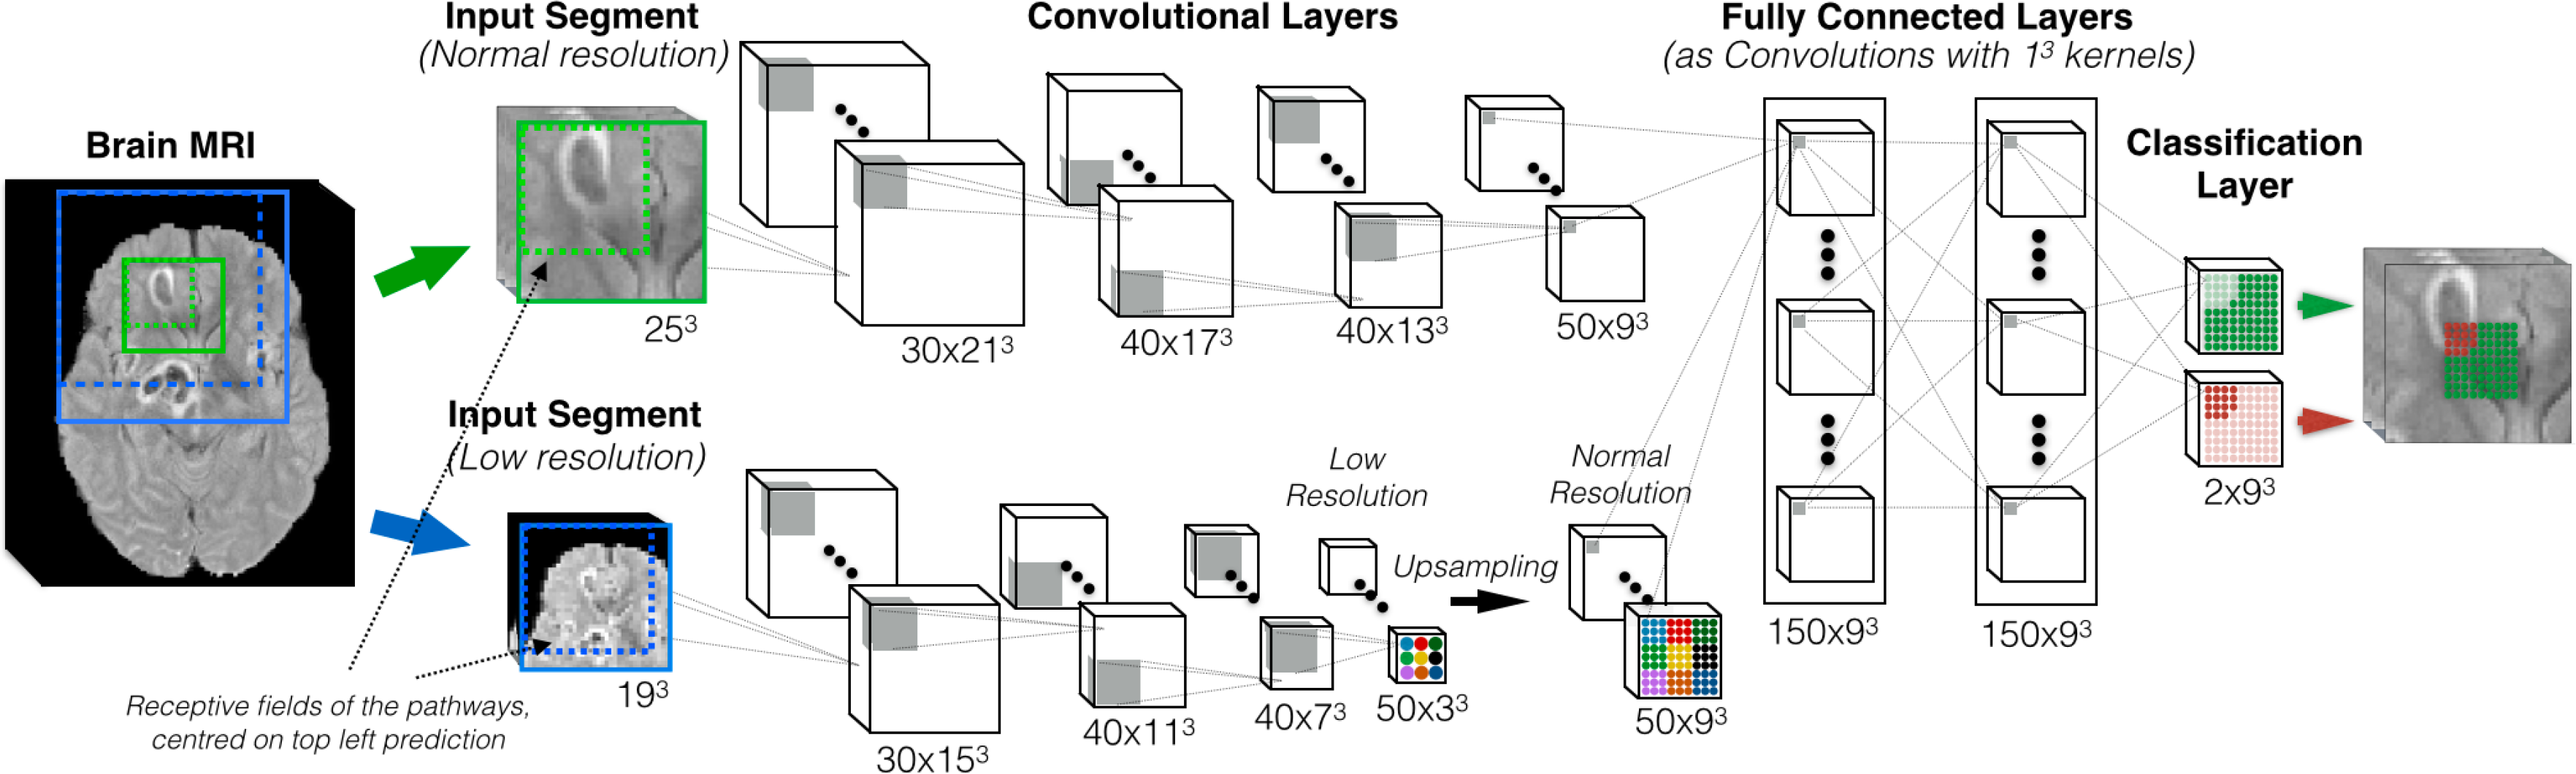
\includegraphics[width=\textwidth]{images/deepmedic}

  \caption[DeepMedic 3D CNN model]{
    DeepMedic 3D \acrshort{CNN} model for brain lesion segmentation \cite{neural:3d-cnn-crf}
    \label{fig:deepmedic}
  }
\end{figure}

Another application of 3D \glspl{CNN} has been in action detection and segmentation for videos.
In this case video imaging was treated as a 3D image where the 3rd dimension represents
time.
~\cite{neural:3d-cnn-action-detection}

On the \gls{PMHNK} dataset some results have already been obtained. By using the \gls{CT} scans and
extracting some features. In this case, the extracted features were:
\begin{itemize}
  \item First order statistics: Energy
  \item Shape: Compactness
  \item Gray level run length: Gray level non-uniformity
  \item Wavelet (HLH) 
\end{itemize}
By fitting the features through a \gls{CPH} model a \gls{CI} of 0,628 was obtained for the whole
dataset.
~\cite{medical:ct-based-radiomic-signature}

\ssecc{Problem Formulation}

This problem is centered around survival prediction and it will be using the \gls{PMHNK} dataset. 
As it has been previously said, the current results for the dataset is a \gls{CI}
of 0,628 \cite{medical:ct-based-radiomic-signature} by using four different features.
The problem statement will be as follows:
\begin{quotation}
  Can a better survival prediction than the current results, be obtained using imaging data and
  \gls{DNN}?
\end{quotation}

\ssecc{Objectives}
\label{sec:objectives}

The objectives to achieve will be:
\begin{itemize}
  \item Get a better understanding of survival prediction problems.
  \item Be able to analyze the \gls{PMHNK} dataset to get different strategies for building a 
  deep learning model.
  \item Develop a new deep learning model to improve the survival's prediction rate of
  \gls{PMHNK} dataset patients compared to models built on traditional radiomic features.
  \item Investigate and compare the performance of the deep learning-based method to 
  the more conventional methods, such as hand-engineered radiomic features.
  \item Get a better \gls{CI} than the \emph{volume} feature, which is often used in clinic as a
  prognostic feature, its \gls{CI} is 0,628.
\end{itemize}

\ssecc{Stakeholders}

\sssecc{Developer}
Is the person in charge of the research, document and implement all the required software.
In addition he is responsible for the project management and the writing of the report
and all the required documentation. This actor works as agreed with the director and
he is, ultimately, the person in charge of accomplishing the deadlines.

\sssecc{Director}
The project will be directed by professor Benjamin Haibe-Kains, from the Bioinformatics 
and Computational Genomics Laboratory. He is the main responsible for guiding, giving 
advice and, in general, helping the developer.
His action is key to determine possible errors in the project, both in its proposal and 
execution.
~\cite{bhklab}.

\sssecc{Beneficiaries}
The project beneficiaries will depend on its outcome. If a more efficient model is found, the
beneficiaries will be the researchers trying to test a new cancer treatment method. Moreover,
the final patient will also be benefited because more modern research techniques will be used.

However, if a more efficient model is not found, the beneficiaries will be future researchers
trying to find the best model for survival analysis, since this would prove which 
methods do not work well for this problem.

\ssecc{Scope}

This project will be centered around the \gls{PMHNK} dataset. This dataset will be analyzed
and a model will be created accordingly.

Since the project aims to create a \gls{ML} model, the first task will be to learn and 
to understand how Neural Networks work. Also, since the inputs will have imaging data, learning
how \gls{CNN} work will be necessary too, as they are really useful for analyzing them. 
This way, I will have a fully understanding of the 
background that all these methods use to create models for survival prediction.

The following task will be to understand how survival prediction problems are approached. An
example of survival prediction is the \emph{DeepSurv} python package, so being able to set 
up, to run and to understand the package will give me a bit more of background in the problem.
However, \emph{DeepSurv} uses a \gls{CPH} model but in this case an attempt will be made to use
a different model, since a \gls{CPH} model is only valid under certain circumstances.
~\cite{medical:deep-surv-github, medical:cox}

Afterwards, a deep learning model will be created, starting from zero but trying to use some
ideas from other completed projects. The model, unlike \emph{DeepSurv}, will not be using
the \gls{CPH} model. In this case, the approach will be to directly optimize the \gls{CI}
instead of get a better prediction of the hazard function \( \lambda(t) \) to optimize 
the \gls{CI}.

To directly optimize the \gls{CI} the comparison of two pairs will be predicted instead. So,
for a pair of two patients \( A \) and \( B \) the model should predict if \( T_A < T_B \),
where \( T \) stands for survival time. So the output should be \( 1 \) if the condition holds
\texttt{true} and \( 0 \) otherwise.

To do so, a siamese neural network will be used,
this type of networks are best suited to compare similarity between the inputs and is usually
used for tasks such as face recognition. Since it will be used to compare a pair's survival
time and not similarity, some changes should be made before using the network.

\ssecc{Methodology}

This project is part of a research project at Benjamin Haibe-Kains Bioinformatics and 
Computational Genomics Laboratory \cite{bhklab}. This means that every week there will be a 
laboratory meeting where different members will be presenting their progress and feedback will
be received accordingly. Once in a while this project's progress will be presented there.

Moreover, a weekly meeting with the Principal Investigator will be scheduled to discuss
the progress made. This weekly meeting should help in determining possible errors during the 
project's development and provide further guidance.

Also, since fitting a machine learning model is not a straightforward task, this means that 
it will require a process of trial and error until the proper solution is found. 
So, during this process, tasks will be assigned on a weekly basis with the objective to
improve the results from the previous ones.

\ssecc{Possible obstacles and solutions}

\sssecc{Training time}

Since this project involves \gls{CNN}, the training time can be a problem. 
The convolution operation is computationally expensive so, depending on the network, the 
training time can be of several days. Usually this type of networks are trained using 
\glspl{GPU} since the convolution operation can be performed faster in this type of processor. 
Also, while just inferring the values does not require
much power, training needs a lot more power. 

To solve this problem, the training will be done at \gls{CC} a computing facility which 
has multiple computing clusters with \glspl{GPU}. \gls{CC} provides access to two different 
clusters:
\begin{itemize}
  \item \emph{Cedar} Has a total of 58.416 \acrshort{CPU} cores and 584 NVIDIA P100 
  Pascal \glspl{GPU} for computation. The complete cluster specification can be found at
  \url{https://docs.computecanada.ca/wiki/Cedar}
  \sloppy
  \item \emph{Graham} Has a total of 35.520 \acrshort{CPU} cores and 320 NVIDIA P100 
  Pascal \glspl{GPU} for computation. The complete cluster specification can be found at
  \url{https://docs.computecanada.ca/wiki/Graham}
\end{itemize}

Both clusters use a queue system managed through Slurm Workload Manager \cite{tool:slurm}. 
The queuing system has a score and it lowers the score based on the resources that have been
used. The lower the score the less the priority a job has to be executed into the cluster.
This means that, when using the cluster, requesting too much or unnecessary resources should be 
avoided.

\sssecc{Monitoring Tools}

The work will be done with the help of Git and GitHub. This tools will help monitoring
the project's evolution. The purpose of Git is to be able to do small revisions,
named commits, and to document all the different changes in the project. Also, it's 
prepared to allow multiple contributors in the same project. Moreover,
Git projects can be stored in a server, GitHub it's an online platform that allows
remote Git repositories. GitHub has integrated an issue system, a milestone system
and it's really integrated with Git's contributor system.
~\cite{tool:git, tool:github}

\sssecc{Bugs}

Considering the software development process, it's no big surprise that it's really easy to
introduce bugs while writing or modifying the source code. To ensure no bugs are present,
some unit tests will be written to check if the model is still giving correct results.
However, this will be a difficult task since it's not easy to check whether a deep 
learning model is just overfitting or that it's giving wrong results.

\sssecc{Scheduling}

Although four months seems plenty of time, spending more time than estimated in a single task
can happen. To avoid this problem weekly meetings will be scheduled with my Principal Investigator
to see which is the best way to continue to keep on track, to reconsider or adapt planification.

\sssecc{Not enough data}

Since the starting dataset is quite small (\( \sim 500 \) samples) overfitting may be a problem
and different methods should be used to avoid it. The possible solutions are:
\begin{itemize}
  \item Using regularization to avoid units with a very high weight.
  \item Using dropout to force each unit to learn with only part of the data, and thus generalize.
  \item Using data augmentation techniques such as random crops or random rotations to increase
  the number of images in the dataset.
\end{itemize}
